\documentclass[compress,10pt]{beamer}
\setbeamertemplate{background canvas}[vertical shading][bottom=white,top=structure.fg!25]
\usetheme{Hannover}
\setbeamertemplate{headline}{}
\setbeamertemplate{footline}{\today -- FEMTO-ST, Besan\c con}
\setbeamersize{text margin left=0cm}

\setbeamertemplate{navigation symbols}{}
\graphicspath{{../linux_mag/misc_gps/}{/home/jmfriedt/sdr/b210/190129_gps_2046kHz/}}

\usepackage{url,verbatim,amsmath,listings}
\usepackage{bm}

\definecolor{mygreen}{rgb}{0,0.6,0}
\setlength{\footnotesep}{0.cm}

\beamertemplatenavigationsymbolsempty


\usepackage{listings,multicol}
\usepackage{color}

\definecolor{grey}{rgb}{0.95,0.95,0.95}
\definecolor{red}{rgb}{1.0,0.0,0.0}
\definecolor{green}{rgb}{0.0,0.6,0.0}
\definecolor{blue}{rgb}{0.0,0.0,1.0}
\lstloadlanguages{bash,Java,C,C++,csh,make,sh}%%[Visual]Basic,xml}
\lstset{frame=none,basicstyle=\footnotesize,breaklines,tabsize=2,captionpos=b,prebreak={\hbox{$\rightarrow$}},postbreak={\hbox{$\hookrightarrow$}},showstringspaces=false,backgroundcolor=\color{grey}\bfseries,keywordstyle=\color{blue},commentstyle=\color{green}\textit,stringstyle=\color{red}\ttfamily,abovecaptionskip=2pt,aboveskip=0pt,belowskip=0pt,belowcaptionskip=0pt}
%\lstset{moredelim=[is][\color{red}]{_+_}{_+_}}

\beamertemplatefootpagenumber


\title[FPGA]{Spoofing GPS \\
{
is it really the time we think it is, and are we really where we think we 
are ?}
 \vspace{0.2cm}}
\author[]{G. Goavec-Merou$^1$, J.-M Friedt$^1$, F. Meyer$^2$\\ \ \\
$^1$ FEMTO-ST Time \& Frequency, Besan\c con, France\\
$^2$ Besan\c con Observatory, Besan\c con, France\\
\vspace{0.3cm}
%\hspace{-2.92cm}
%\parbox{1\linewidth}{\includegraphics[height=4.38cm]{150924_1_map1}~
%\includegraphics[height=4.38cm]{151001_map1}}\\
%\hspace{-1.5cm}Sept. 24th, 2015\hfill Oct. 1st, 2015\hfill\\ \ \\
slides at \url{jmfriedt.free.fr/fosdem2019_gps.pdf}\\\ \\
sequel to ``Software Defined Radio for processing GNSS signals (FOSDEM 2015)''
}

\definecolor{grey}{rgb}{0.95,0.95,0.95} 
\lstloadlanguages{C}
\lstset{numbers=none,frame=none,basicstyle=\tiny,breaklines,tabsize=2,captionpos=b,prebreak={\hbox{$\rightarrow$}},postbreak={\hbox{$\hookrightarrow$}},showstringspaces=false,backgroundcolor=\color{grey}\bfseries,keywordstyle=\color{blue},commentstyle=\color{mygreen}\textit,stringstyle=\color{red}\ttfamily,abovecaptionskip=2pt,aboveskip=0pt,belowskip=0pt,belowcaptionskip=0pt}

\begin{document}

\begin{frame}\frametitle{FPGA/CPU co-design training}

CPU/FPGA training (master2 level)

\begin{itemize}
\item Stable {\tt github} repo @ \url{https://github.com/oscimp/oscimpDigital} {\bf with tutorials} explaining
usage of each processing block
\item Linux driver and communication interfaces
\item Devicetree for dynamic definition of resources, driver and bitstream
\item Xilinx IP modification
\item Custom VHDL IP integration
\item OscimpDigital block usage (combined FPGA+Linux driver+userspace co-design)
\item Demonstration on digital phase locking of numerical oscillator
\end{itemize}

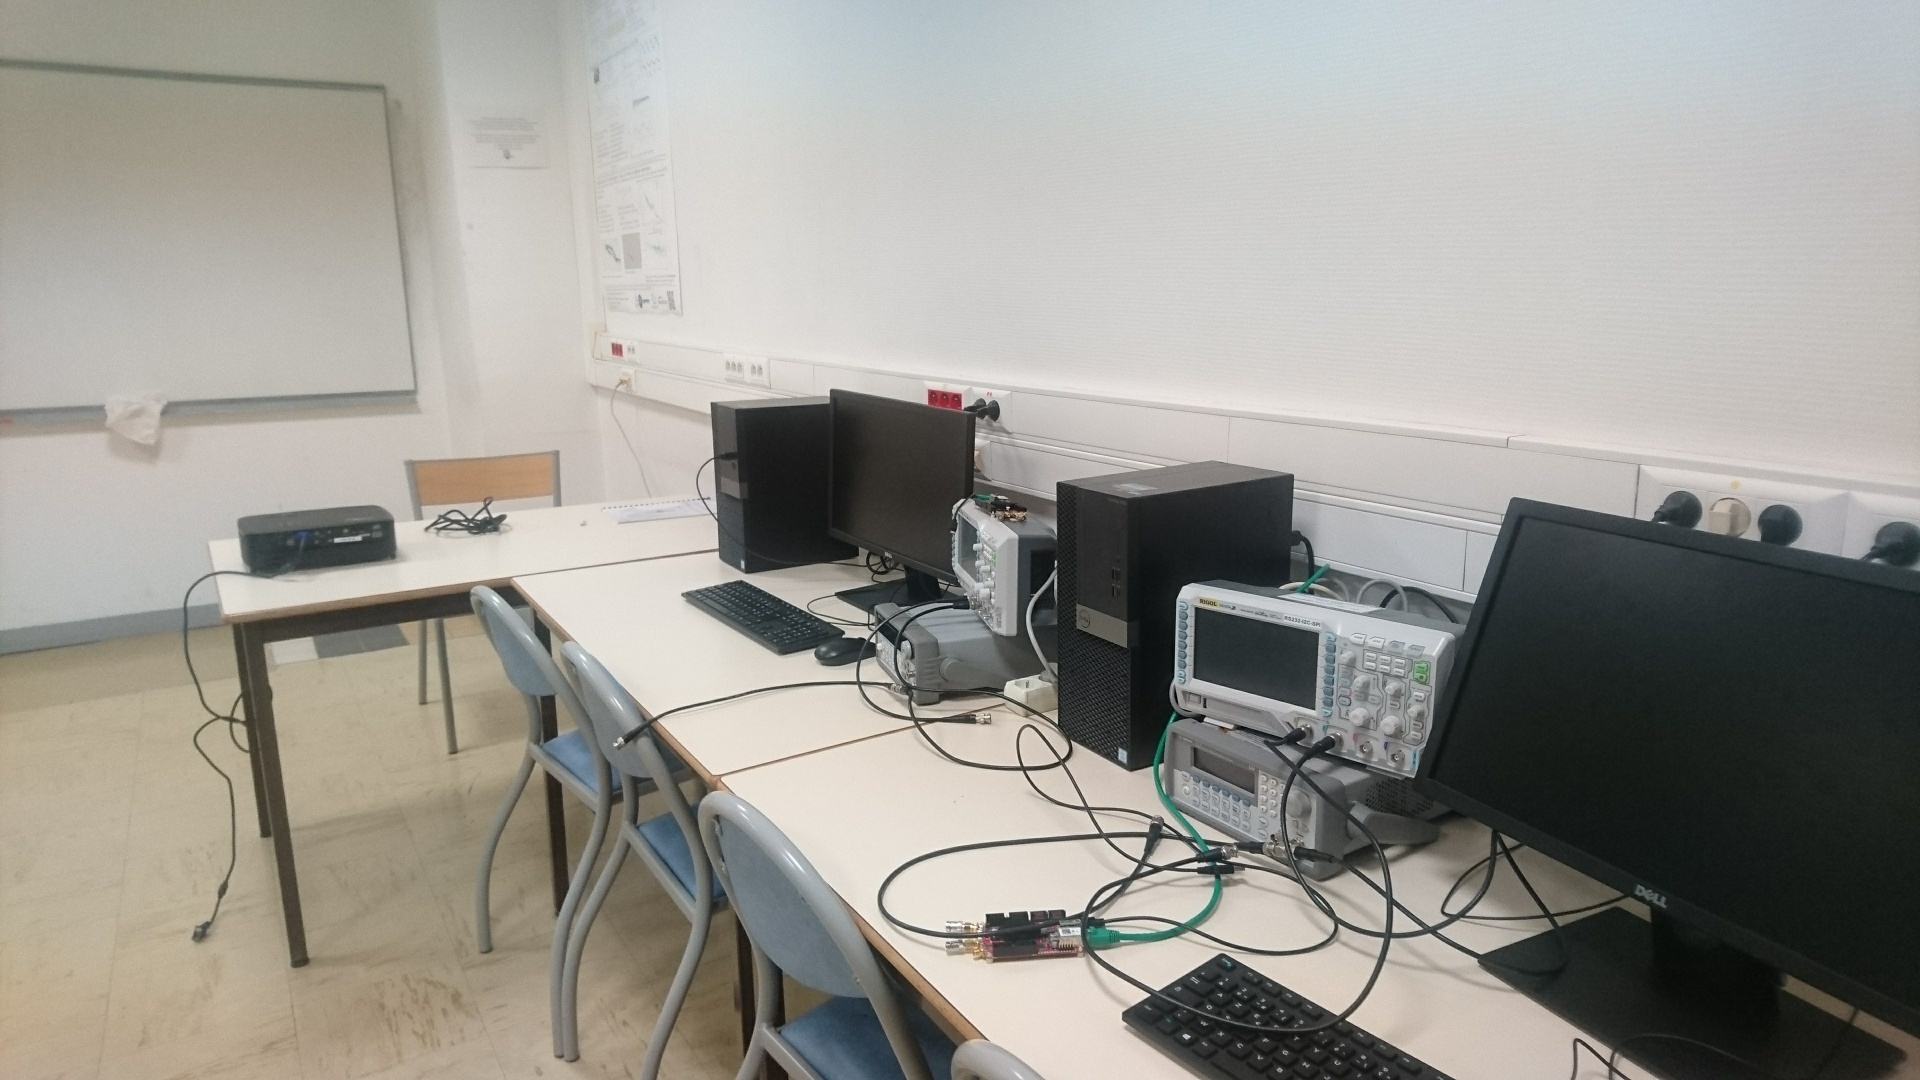
\includegraphics[width=.5\linewidth]{/home/jmfriedt/xilinx/oscimpDigital/DSC_0050.JPG}
\end{frame}

\begin{frame}\frametitle{White Rabbit}

\begin{itemize}
\item
Completed deployment of the ENSMM (hydrogen maser) -- Besan\c con Observatory (cesium clock) -- university (teaching department link)
(started end of July 2018, completed beginning of January 2019)
\item Beyond 1-PPS \& 10~MHz distribution: {\bf using} WR
\begin{itemize}
\item distributed DDS (Ettus Research X310 -- problem communicating over WR)
\item distributed ADC (custom board -- hardly supporting anything)
\item pulse timing (DIO): functional board
\end{itemize}
\end{itemize}

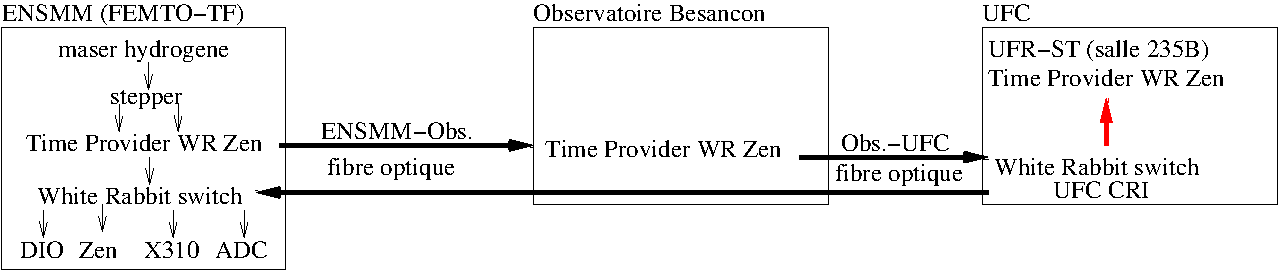
\includegraphics[width=\linewidth]{/home/jmfriedt/femto/labcom_gorgy/190124_WR_fac/architecture.pdf}

Network architecture: from research to teaching centers

\end{frame}
\begin{frame}\frametitle{Teaching timeline}

\vfill

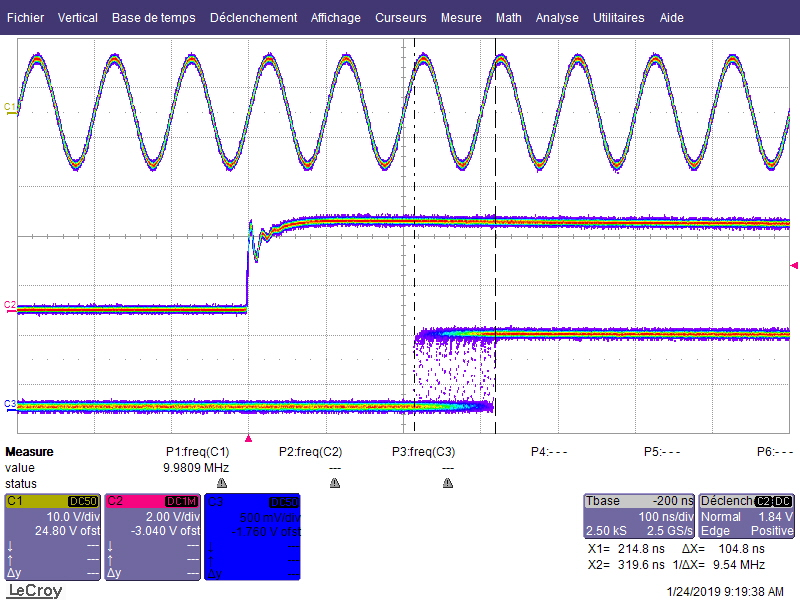
\includegraphics[width=.49\linewidth]{/home/jmfriedt/femto/labcom_gorgy/190124_WR_fac/spi2} % round trip statistics
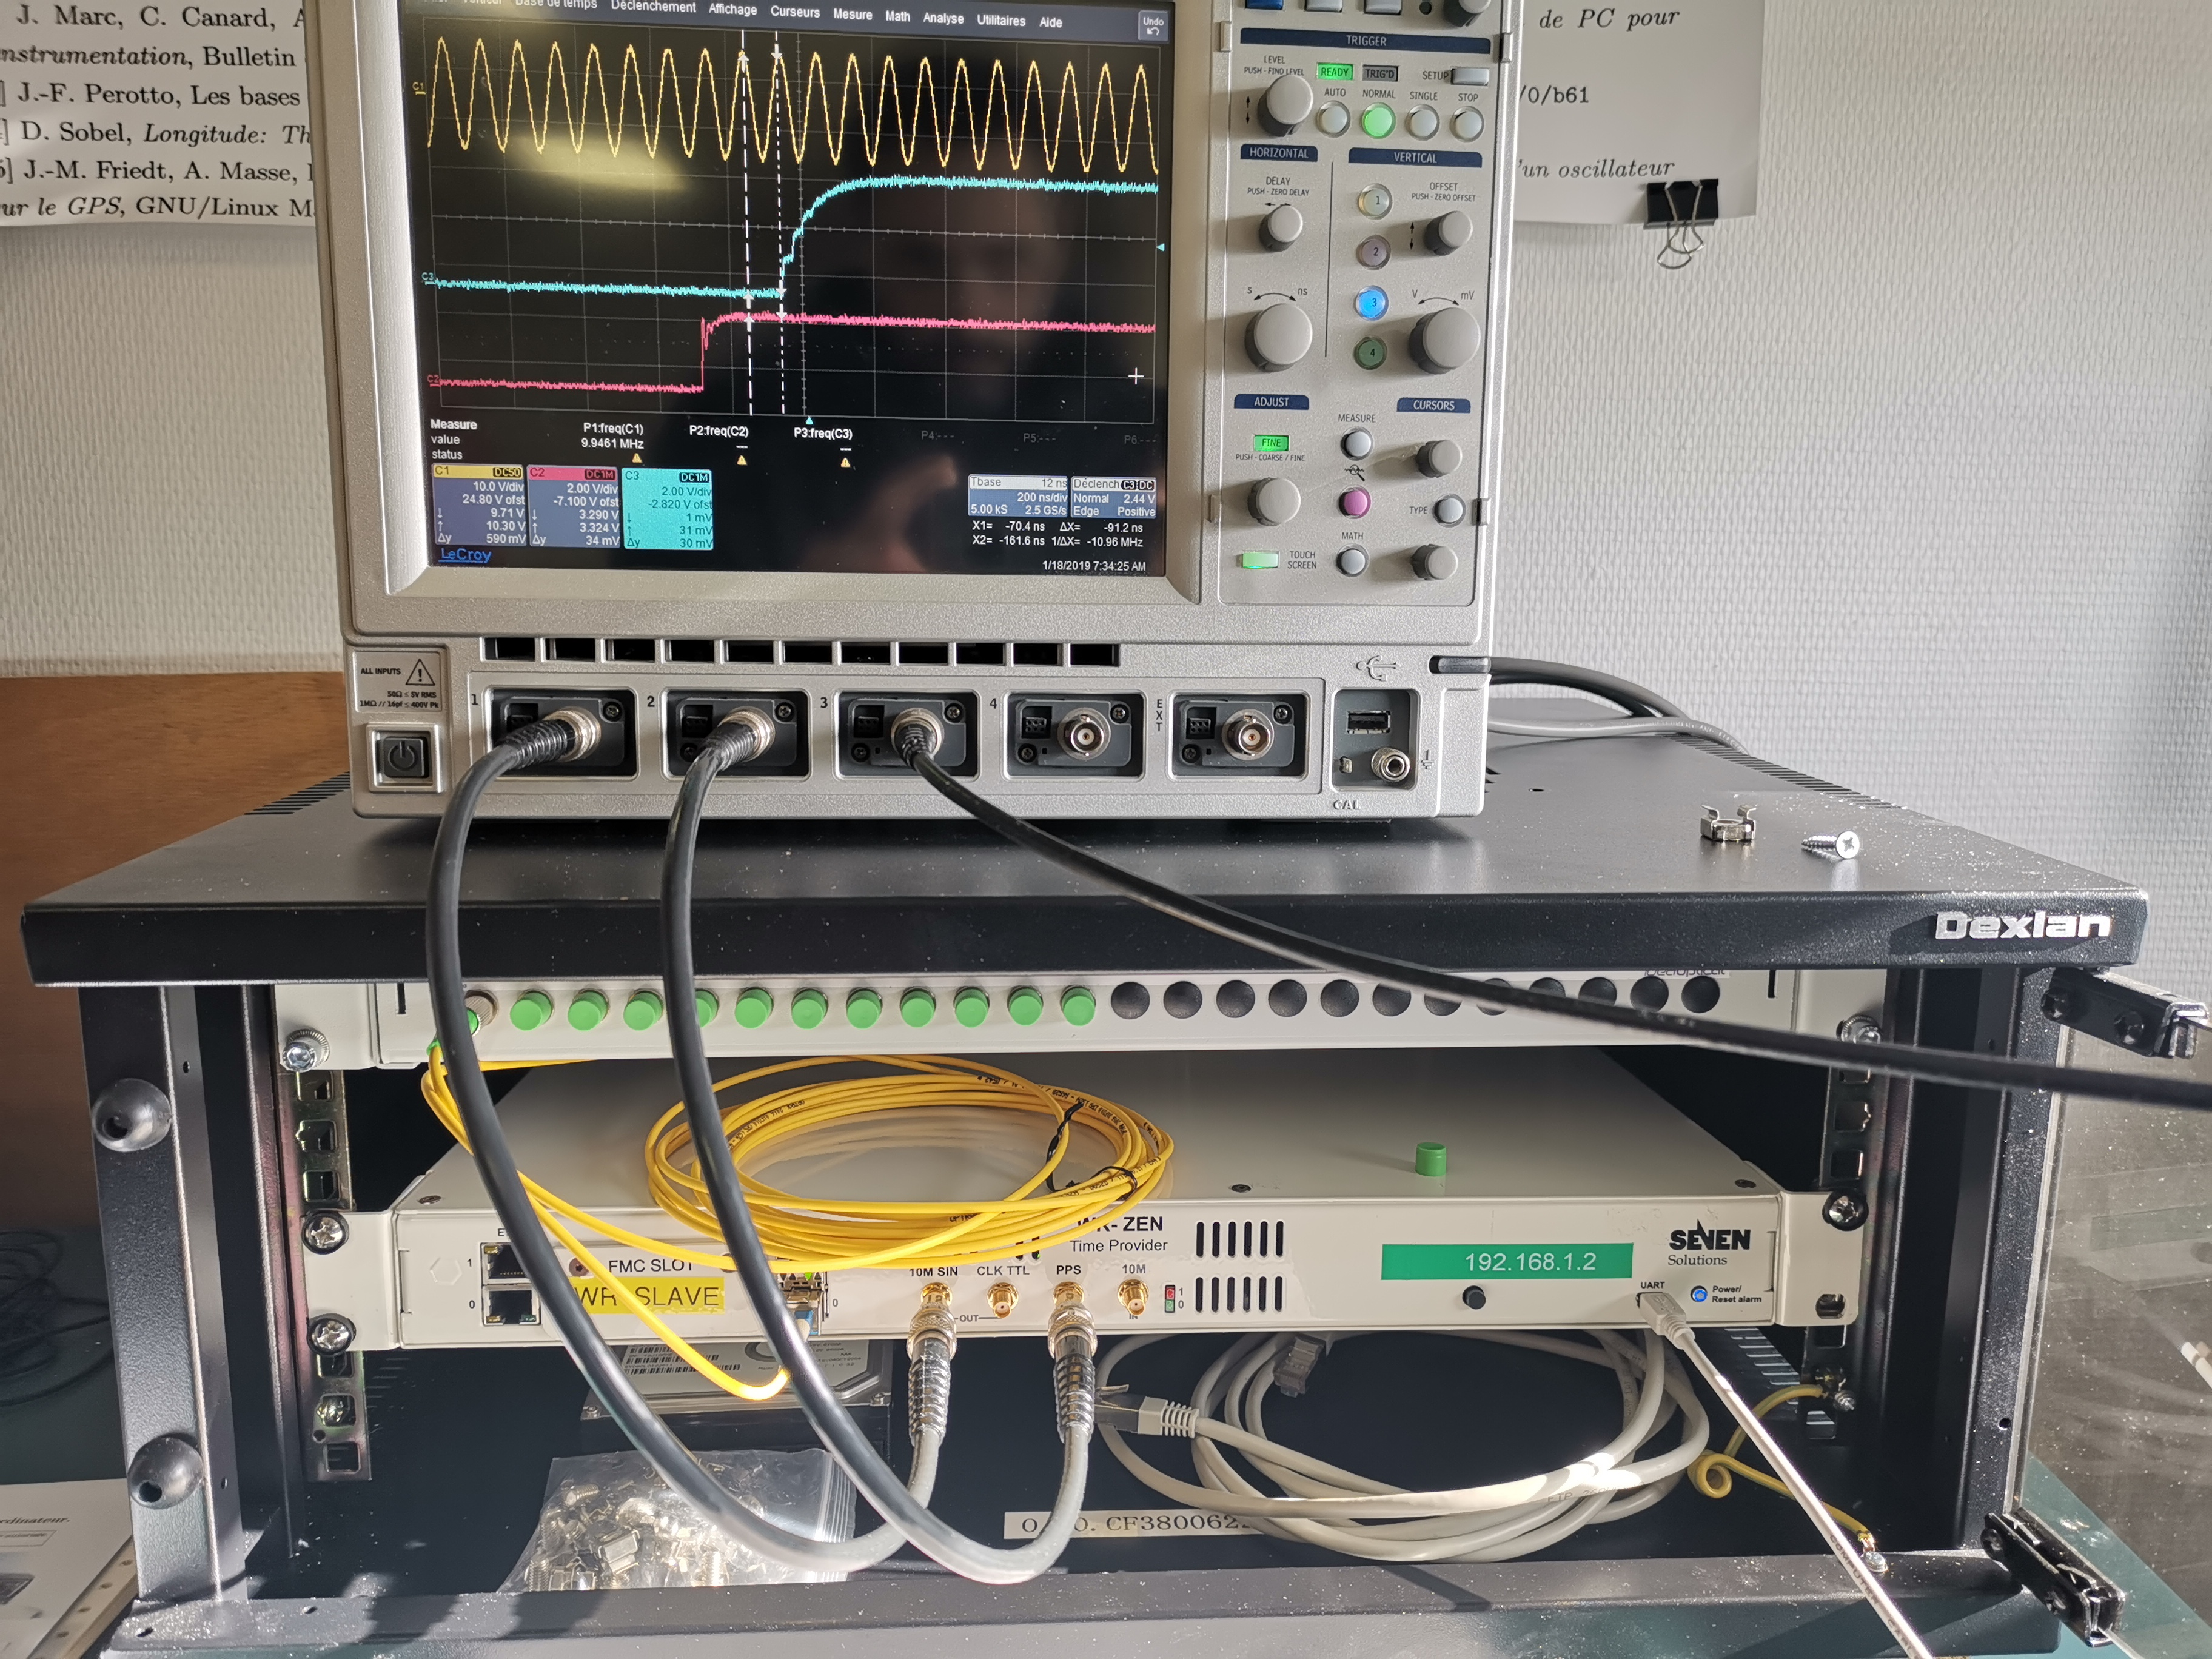
\includegraphics[width=.49\linewidth]{/home/jmfriedt/femto/labcom_gorgy/190118_235B/IMG_20190118_125305.jpg} % 235B setup
\vfill

\begin{itemize}
\item Bachelor: programmable delay line for GPS 1-PPS negative sawtooth delay compensation
\item Master1: WR controlled DDS for distributed RF source (using 10~MHz \& 1~PPS)
\item Master2: distributed ADC, DDS (embedded board tackling PTPv2 signals)
\end{itemize}

\end{frame}
\begin{frame}\frametitle{Digital oscillator lock demonstration}

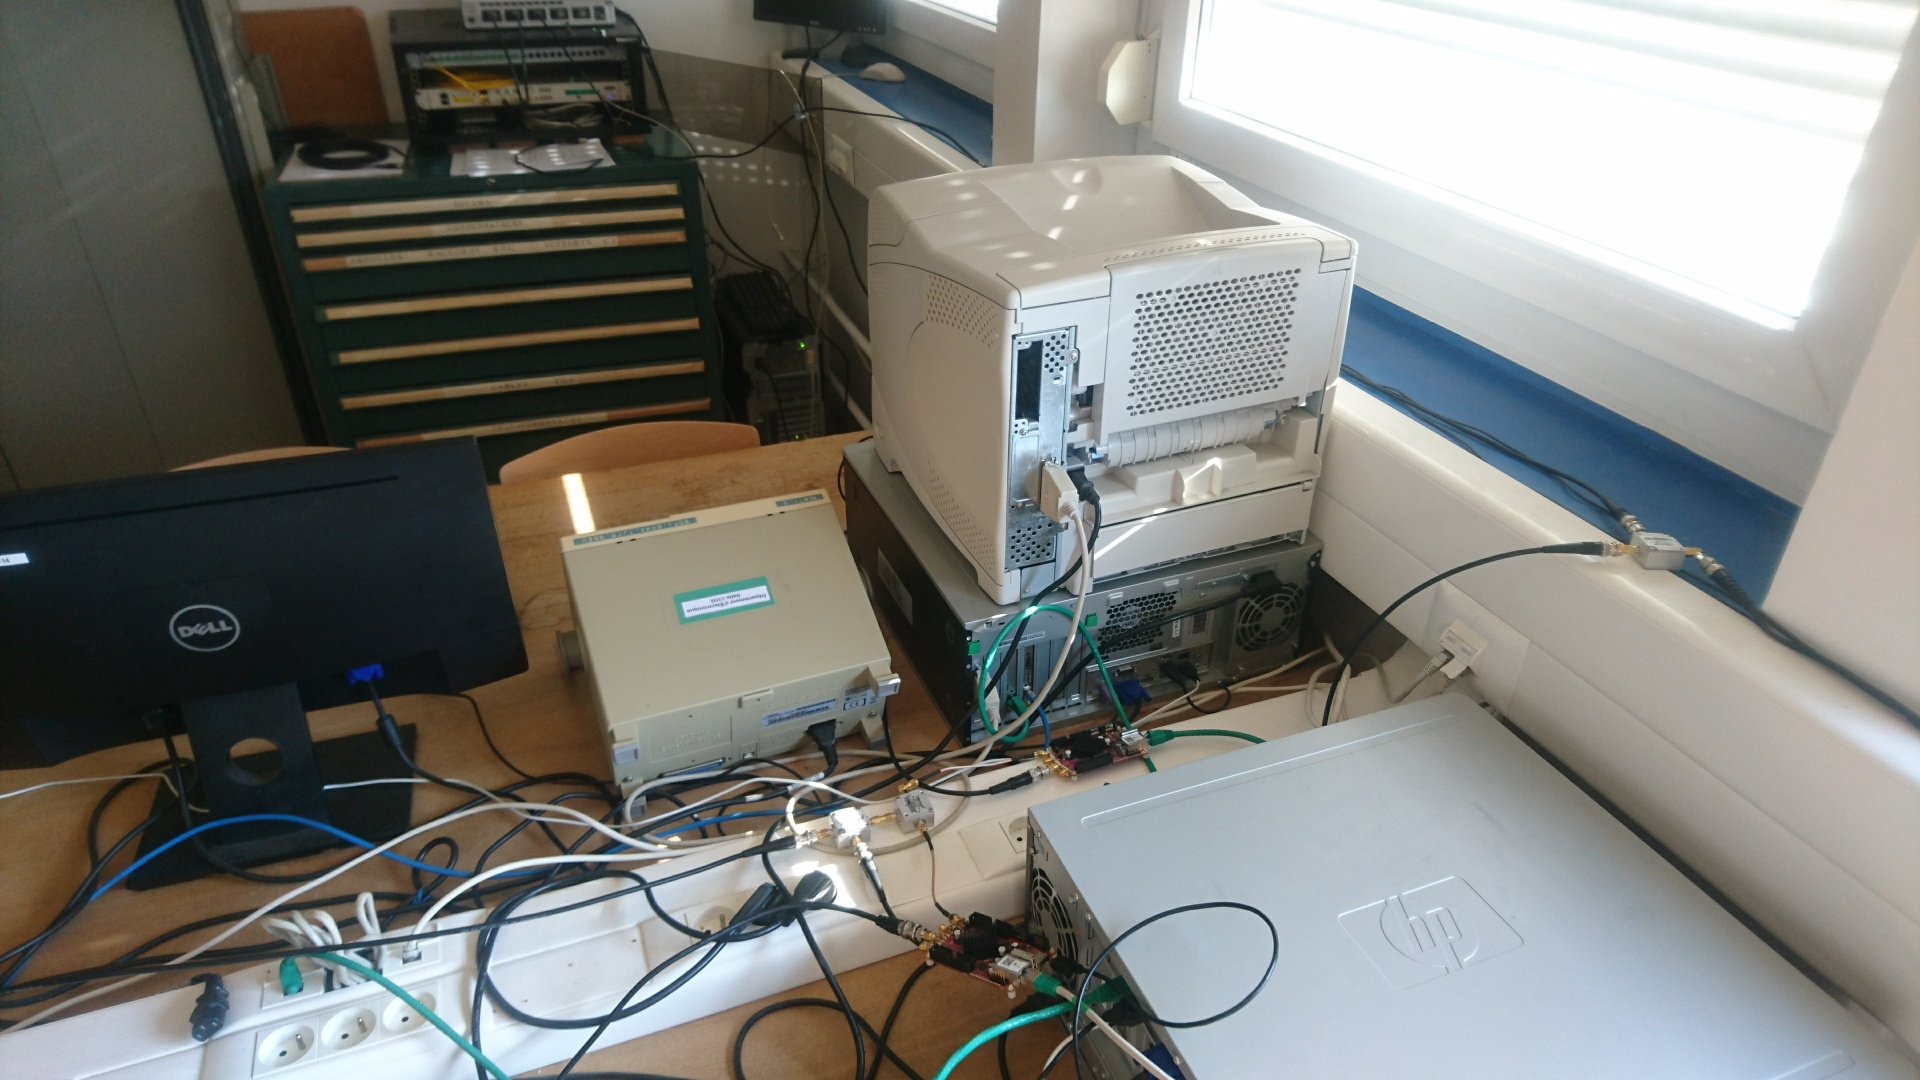
\includegraphics[width=.49\linewidth]{/home/jmfriedt/femto/labcom_gorgy/190124_WR_fac/DSC_0091}
\end{frame}
\end{document}
